\section{Лекция 2.}

\subsection{Геом. смысл дифференциальных уравнений}

\deff{def:} Если каждой точке $(x,y)$ области определения функции $f$ сопоставить вектор, направленный под углом $\arctan f(x,y)$, то получится \deff{поле направлений} $f(x,y)$.

\begin{center}
   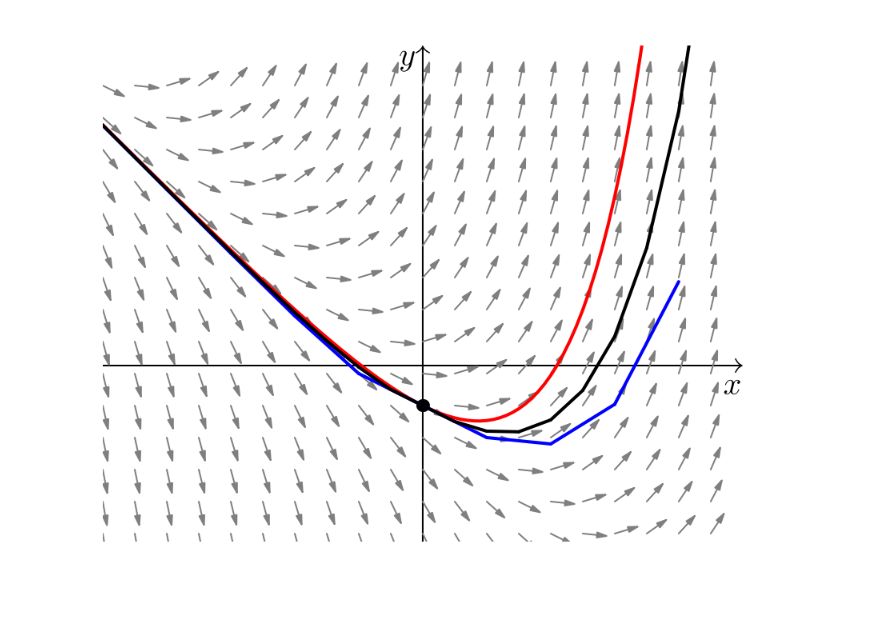
\includegraphics[width=14cm]{assets/2-arrows.png}
\end{center}


Рассмотрим один способ построить  приближение к интегральной кривой. Взяв некоторую точку $(x_0,y_0)$ в качестве начальной, будем двигаться по направлению поля в точке $(x_0,y_0)$ до точки с абсциссой $x_1 = x_0 +h$, ординату которой обозначим через $y_1$. Сделаем то же самое, что много много раз и получим \deff{ломаную Эйлера}. 

\deff{def:} \deff{Изоклиной} $I_k$ уравнения называют множество уровня функции $f$:
$$I_k =\{(x,y)\in dom f | f(x,y) =k\}$$

TODO: метод изоклин 

\subsection{Уравнение в полных дифференциалах.}

\deff{def:} Уравнение 
$$P(x,y)dx + Q(x,y) dy =0$$
называют \textbf{уравнением в полных дифференциалах} в области $G$, если для него существует \textbf{потенциал}, то есть такая дифференцируемая функция $u$, что для всех $x,y \in G$:
$$du = P(x,y)dx + Q(x,y)dy$$

\thmm{Теорема (общее решение УПД)}

Пусть $G \subset \mathbb{R}^2$ --- область, функция $u: G \rightarrow \mathbb{R}$ дифференцируема, $u'_x =P, u'_y =Q$. Тогда функция $y = \varphi(x)$ - решение уравнения УПД на промежутке $E$, если и только если она дифференцируема на $E$ и при некотором $C \in \mathbb{R}$ неявно задана уравнением:
$$u(x,y) = C$$

\textbf{Доказательство:}

\uline{Достаточность.} Дифференцируя равенство $u(x, \varphi(x))=C$ по переменной $x \in E$, находим:
$$u'_x(x,\varphi(x)) + u'_y(x,\varphi(x))\varphi'_x \equiv 0$$
Так как $u'_x = P, u'_y = Q$, то определению функция $\varphi$ является решением

\uline{Необходимость.} На промежутке $E$ верно тождество
$$P(x,\varphi(x)) + Q(x,\varphi(x))\varphi'(x) \equiv 0$$
Левая часть этого равенства совпадает с производной функции $u$ по переменной $x$.


\hfill Q.E.D.

\deff{def:} Уравнение
$$P(x) dx + Q(y) dy=0$$
называют \deff{уравнение с разделенными переменными.}

\deff{Следствие (общее решение УРП):}

Пусть $P \in C(a,b), Q \in C(c,d)$. Тогда функция $y =\varphi(x)$ --- решение уравнения на промежутке $E$, если и только если она дифференцируема на $E$ и при некотором $C \in \mathbb{R}$ и при некотором $C \in \mathbb{R}$ неявно задана уравнением:
$$\int P(x) dx + \int Q(y) dy = C$$
\textbf{Доказательство:} подставим и проверим.


\deff{Утверждение (необходимое условие УПД)}.

Пусть потенциал $u \in C^2(G)$. Тогда:
$$P'_y = Q'_x$$

\thmm{Теорема (признак УПД)}

Пусть $G \subset \mathbb{R}^2$ --- односвязная область $P,Q \in C^1(G), P'_y = Q'_x, (x_0,y_0)\in G$. Тогда уравнение в полных дифференциалах в области в $G$ с потенциалом:
$$u(\overline{x}, \overline{y}) = \integral{\gamma(\overline{x}, \overline{y}))}{}P(x,y)dx + Q(x,y)dy =0$$
